% Chapter Template

\chapter{System Implementation} % Main chapter title

\label{Chapter5} % Change X to a consecutive number; for referencing this chapter elsewhere, use \ref{ChapterX}

\lhead{Chapter 5. \emph{System Implementation}} % Change X to a consecutive number; this is for the header on each page - perhaps a shortened title
In this chapter the implementation of various components specific to the experimental platform taking advantage of the framework proposed in \ref{Chapter4} is presented. The Software is designed using a layered hierarchical structure. The various layers of the system are
\begin{itemize}
\item \emph{Hardware Layer} is composed of sensors and robots connected to the network. Currently only those sensors that support TCP/IP network communication are considered.
\item \emph{Distributed Components Layer} is composed of individual processes that could be running across different computers/devices in the network
\item \emph{Application Components Layer} is the central server of the experimental platform
\item \emph{User Interface} takes the responsibility of providing useful and intuitive user-interface to the end users.
\end{itemize}
The architecture of the system shown in Fig~\ref{fig:architecture}. More finer details of each of the layers are presented in the following Sections~\ref{ssec:app_comp}$\sim$\ref{ssec:ui_comp}.
\begin{figure}
\centering
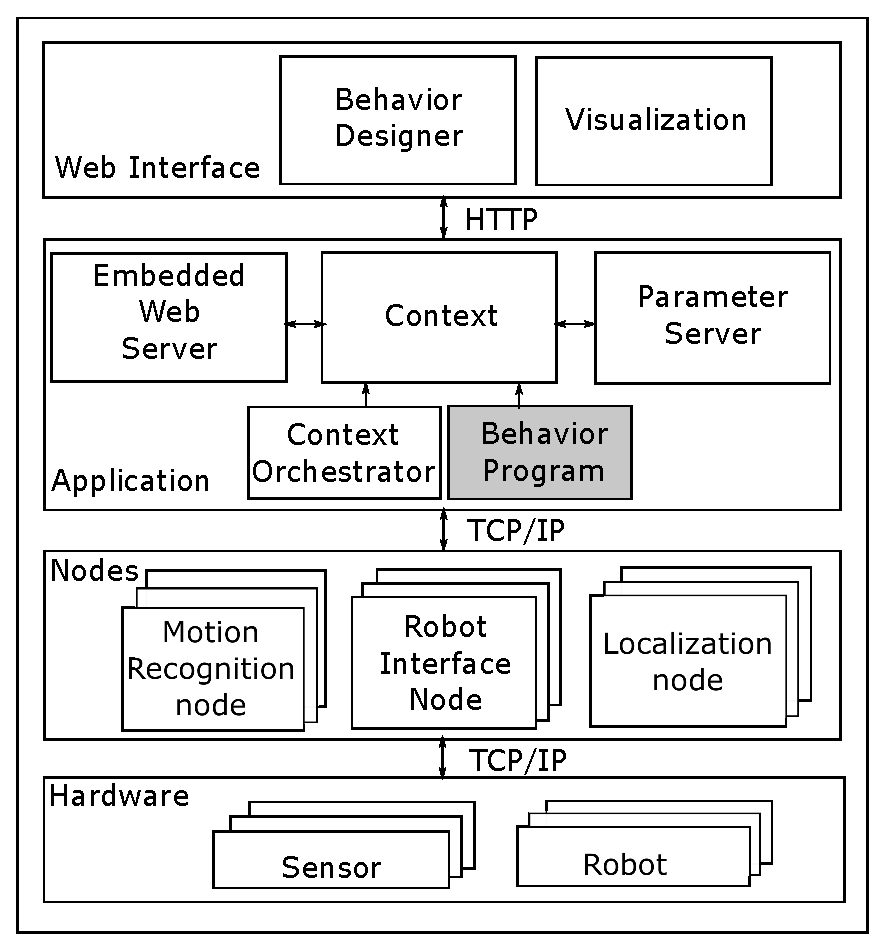
\includegraphics[width=\textwidth]{assets/architecture.eps}
\caption[System Architecture]{System Architecture}
\label{fig:architecture}
\end{figure}
\section{Application Components}
\label{ssec:app_comp}
The application level components are responsible for bootstrapping and maintain the uptodate status of the system. 
\subsubsection{Context}: The application context contains the complete description of the world. It contains latest information about
\begin{itemize}
\item Robot(s): A list of robots in the environment along with their 6D pose, Sensor information like Joint values etc.,
\item Human(s): A list of humans with their Skeleton Positions and Orientation, Active Gestures/Motions
\item Object(s): A list of manipulable objects in the environment along with their properties like description, color etc.,
\item Gesture Modules : A set of gesture recognition modules registered in the system that can actively provide information about the gestures of the humans in the environment.
\item Robot Behavior Modules: A set of robot behavior execution modules registered in the system.
\end{itemize}
The data structure of the context is shown in Fig~\ref{fig:system_context}
\begin{figure}
\centering

\includegraphics[width=\textwidth]{assets/to_be_added.png}
\caption[System Architecture]{System Architecture}
\label{fig:system_context}
\end{figure}
\subsubsection{Parameter Server}: The parameter server acts as a central repository for managing the parameters of the system and of the distributed components.
\subsubsection{Context Orchestrator}: The orchestrator collect uptodate information about the robots and humans in the environment from the perception system and updates the Context. The algorithm used by the Orchestrator to update the context information is shown below.

\subsubsection{Bootstrapper} : The bootstrapper takes care of initializing the system and starting up all the pre-configured nodes. It also takes of starting and stopping the behavior programs when requested by the user. 
\subsubsection{Embedded Web server} : The web server embedded in the application serves the file and data requests from the web client.
\subsubsection{Behavior Program} : A dynamic component that will be created when the user starts the program he/she designed using the user interface. The declarative description of the behavior is parsed in order to create a memory model. The Behavior program node monitors the application context for the motion triggers and invokes the corresponding robot actions according to the way it is being described in the program.
\section{Distributed Components}
\label{ssec:dist_comp}
These are nodes in the system each with a specific goal that can be started/stopped at any time during the entire application life-cycle without affecting the other nodes or the system. All the nodes will communicate with the application using message passing techniques. They can run in any machine inside the network.
\begin{itemize}
\item \emph{Motion Recognition Node} : A dedicated node that interacts with a motion recognition sensor and sends the detected gestures and motions to the application. Additionally each motion recognition module registers a set of actions/gestures that could be detected with the sensor associated with it.
\item \emph{Robot Interface Node} : A dedicated node that interacts with a specific robot and can invoke a set of actions on it. It also sends periodic update about the Robot status to the application. Moreover it registers a set of actions that could be invoked on the robot associated with it.
\item \emph{Localization Node} : A dedicated node which uses the perception system to resolve and publish the current position of the robot and the human which is very important for interaction.
\end{itemize}
\section{User Interface}
\label{ssec:ui_comp}
The user interface is a web application that runs on any latest web-kit browsers supporting WebGL technology. 
\begin{itemize}
\item \emph{Behavior Designer}: The Behavior designer surface could be used by the user to drag and drop the behavior blocks and construct the program using the set of motion capabilities registered by the active motion recognition nodes and the set of robot action capabilities registered by the active robot interface nodes. The behavior designed using the designer will be encoded into a declarative XML format and sent to the server when the user request to start the program. The designer offers a full range of capabilities like Create/Edit/Delete/Save behavior programs.
\item \emph{Visualization}: The visualization could be used to see the interaction of the human and robot inside a virtual 3D environment.
\end{itemize}

\begin{algorithm}
 \KwData{Marker\_size, Cube\_size, MDH\_Params}
 \KwResult{TORSO\_POSE}
 \textbf{\emph{Init}}:\;
 k\_model := INIT\_MDH\_PARAM(MDH\_Params)\;
 m\_model := MARKER\_MODEL(Marker\_size, Cube\_size)\;
 \While{True}{
 	data = READ\_SENSOR()\;
 	marker\_poses = DETECT\_MARKERS(data)\;
 	$^{W}{T}_{M}$ = TRANSFORM\_TO\_TOP\_FRAME(marker\_poses, m\_model)\;
 	[$head_{yaw}$,$head_{pitch}$] = READ\_JOINT\_VALUES()\;
 	$^{T}{T}_{M}$ = COMPUTE\_TOP\_FRAME(k\_model,$head_{yaw}$,$head_{pitch}$)\;
 	$^{W}{T}_{T}$ = $^{W}{T}_{M} \times {^{T}{T}_{M}}^{-1}$\;
 	TORSO\_POSE = MEDIAN\_FILTER($^{W}{T}_{T}$)\;
 	PUBLISH(TORSO\_POSE)\;
 }
 %\caption{Localization Algorithm}
 %\label{alg:localize}
\end{algorithm}

% Motion recognition
\begin{algorithm}
 \KwData{Gesture database}
 \KwResult{Gesture Triggers}
 \textbf{\emph{Init}}:\;
 \quad gestures = READ\_DATABASE() \;
 \quad REGISTER\_GESTURES(gestures) \;
 \While{True}{
 	skeletons = GET\_SKELETONS() \;
 	gesture = DETECT\_GESTURE() \;
 	\If{detected}{
 	PUBLISH(gesture) \;
 	}
 	PUBLISH(skeletons) \;
 }
 %\caption{Localization Algorithm}
 %\label{alg:localize}
\end{algorithm}

% Simulation Node
\begin{algorithm}
 \KwData{simulation\_config}
 \textbf{\emph{Init}}:\;
 \quad INIT\_SIMULATION\_ENGINE(simulation\_config) \;
 \quad INIT\_SUBSCRIBERS(simulation\_config) \;
 \quad LOAD\_ENVIRONMENT(simulation\_config) \; 
 \While{True}{
 	sensors = READ\_SENSOR\_VALUES() \; 
 	skeletons = READ\_SKELETON\_DATA() \; 
 	RENDER(robot,sensors)
 }
 %\caption{Localization Algorithm}
 %\label{alg:localize}
\end{algorithm}